\chapter{Asking Billionaires If They Pay Taxes?}

This chapter follows a \emph{School of Hard Knocks} street interview and treats it as a sequence of commercial problems rather than a mere montage of luxury. There is no blackboard here. The mathematics is verbal: a tax heuristic, a distinction between revenue and earnings, a few reported exit values, a nine-step business algorithm, and a final cost equation that behaves like a compact lesson in margin. Curated for note form by LazyingArt LLC, these notes keep the transcript's order and preserve the lecture's central tension: we first ask how wealth is made, and only then ask what happens to it when taxes arrive.

\section{Opening Setup: London as a Tax Laboratory}

The lecture begins with a cold-open promise of scale. We hear about a channel with \(21\) million followers, a reported history of interviewing billionaires, exits measured in billions, and tax bills measured in the hundreds of millions. The montage is not yet an argument. Its function is to place us inside a world where the numbers are large enough that the question of taxation cannot be treated as a side remark.

The host then resets the frame and states the experiment more carefully. London is chosen not only because it is rich, but because it is described as heavily taxed. The basic motivational arithmetic is deliberately rough:
\begin{equation}
T_{\mathrm{heuristic}} \approx 0.45Y,
\qquad
Y_{\mathrm{after}} \approx 0.55Y.
\end{equation}
Here \(Y\) denotes pre-tax money and \(T_{\mathrm{heuristic}}\) is only the host's opening simplification. The point is not tax-law precision. The point is to establish the emotional scale of the problem: at that rate, taxation feels close to taking half.

Before we go further, we need a distinction that the transcript itself forces on us. Throughout the lecture, different people speak about different quantities:
\begin{itemize}
\item \(R\): revenue,
\item \(E\): money ``made in a single year,'' when the speaker does not explicitly say revenue,
\item \(V_{\mathrm{exit}}\): exit value or sale value of a company,
\item \(T\): taxes paid.
\end{itemize}
If we do not keep these objects separate, the interview collapses into hype. If we do keep them separate, a real commercial structure begins to appear.

\section{Rejection as Method and the Move to Mayfair}

The next beat matters more than it first appears to matter. The host tries repeatedly to stop wealthy passers-by, and repeatedly fails. That sequence of refusals is not filler. It is the lecture's first methodological lesson: access to the rich is itself scarce, and therefore the evidence will be noisy, opportunistic, and socially filtered.

Only after that does the lecture pivot. The host announces a change of procedure and heads to Mayfair, described as a place where millionaires and billionaires cluster. In effect, the lecture moves from a random sample to a more concentrated one. We are not yet doing formal probability, but the logic is recognizable: if the subjects are hard to reach, then one should go where the prior density is higher.

The same point returns later in a sharper form as a business principle. But here, at the level of narrative, it first functions as a search rule: when direct access fails, change the geometry of the search.

\section{Case Study I: The Jeweler, the Hypercar, and the Discipline of Reputation}

The first substantial case study begins with the sight of a spectacular car and then immediately destabilizes that spectacle. The interviewee says, in effect, that if we think the car alone defines wealth, then we have misunderstood the matter. He identifies himself as a jeweler and narrates a path that runs from watching people hustle, to buying and selling, to watches, and then from watches to hypercars.

A first numerical anchor appears when he gives the current price of the car:
\begin{equation}
V_{\mathrm{car}} \approx 4.5\times 10^{6}\ \mathrm{GBP}.
\end{equation}
But the more important arithmetic is not the car's sticker price. It is the arithmetic of a luxury cycle. He reports that during COVID he could sell very high-end watches in large enough volume that a single year reached roughly \(25\) million dollars. If we isolate only the spoken watch prices and weekly quantities, we get
\begin{align}
p_{\mathrm{watch}} &\in [700,800]\times 10^{3}\ \mathrm{USD},\\
q_{\mathrm{week}} &\in \{2,3\},\\
R_{\mathrm{week}} &= p_{\mathrm{watch}}\,q_{\mathrm{week}}
\in [1.4,2.4]\times 10^{6}\ \mathrm{USD}.
\end{align}
This is a gross weekly sales flow reconstructed from the transcript. It is not the same object as yearly earnings. The lecture does not give enough detail to identify margins, inventory turns, or overhead. Still, the order of magnitude is clear.

The commercial moral of this first case is not merely that luxury can be profitable. It is that trust enters as a governing constraint. The interviewee says, repeatedly, that word is everything, that broken promises require compensation, and that uncorrected breaches terminate future business. In other words, reputation is not ornament here. It is a repeated-game enforcement mechanism.

His second major claim is biographical rather than financial. He marks fatherhood as the turning point at which growth becomes obligation. That move matters because the lecture does not present financial freedom as a static endpoint. It presents it as something that intensifies once another person depends on us.

\subsection{Question \& Answer}

\paragraph{Question.} Is there a tax hack?

\paragraph{Answer.} The interviewee's answer is emphatically negative in the narrow, illicit sense. There is no ``hack'' that one should rely on. Try to hack taxes and one goes to jail. But that answer is immediately qualified. There are still ordinary expenses, and many people fail to recognize how much of day-to-day commercial life can legitimately be accounted for as expense. The lecture therefore separates two ideas that are often lazily merged: illegal evasion on the one hand, and lawful deduction or expense recognition on the other.

The section closes with a harsher social thesis: the interviewee treats poverty, in many cases, as a consequence of choice and overspending rather than pure fate. The notes should preserve that claim as his rhetoric, not as neutral doctrine. What matters for the chapter's structure is that the host then recaps the segment and sharpens its lesson. Wealth, he suggests, is tied to agency, repeated exposure to opportunity, and the willingness to keep going after getting hit.

\section{Case Study II: Richard Harpin and the Unsexy Business}

The Richard Harpin interview changes the register of the lecture. With the jeweler, we remained near hustle, luxury, and reputation. With Harpin, the lecture turns toward procedure. The surprise is immediate: the business is plumbing and home services, and yet the reported sale value is enormous. The point is to break the audience's attachment to glamour as a precondition for scale.

The transcript gives the central pair of numbers quite plainly:
\begin{equation}
V_{\mathrm{exit}} = 4.1\times 10^{9}\ \mathrm{GBP}
\approx 5\times 10^{9}\ \mathrm{USD},
\qquad
T_{\mathrm{paid}} \approx 1.0\times 10^{8}\ \mathrm{GBP}.
\end{equation}
Again we must keep categories straight. The first quantity is company sale value. The second is tax paid at exit. Neither number is a description of annual operating revenue.

The interview then steps backward and asks where the ambition came from. Harpin frames it through family history, the Great Depression, civil-service caution, and a childhood encounter with visible industrial wealth. What matters structurally is that the lecture does not move from large numbers directly to advice. It first asks how a taste for enterprise gets formed.

Only then does the key reframing arrive: one does not need to invent the next Google. One can take an unsexy business, understand its model, and build scale there. This is the lecture's decisive move from anecdote to method.

\subsection{Question \& Answer}

\paragraph{Question.} Must one invent something radically new in order to become very wealthy?

\paragraph{Answer.} Harpin's answer is no. We are taught in school that copying is a vice, but in business, he says, the better rule is to copy a business model and then improve it slightly. The lecture is not celebrating plagiarism. It is rejecting the superstition that novelty is the only route to magnitude. The relevant contrast is between reinventing the wheel and operating a proven model with greater discipline.

\section{The Nine-Step Algorithm}

Once this point has been made, the lecture finally allows itself a more formal shape. Harpin names a nine-step path to making a billion. We should preserve the order because the sequence is part of the meaning.

\begin{definition}
Let
\[
S=(s_1,\dots,s_9)
\]
denote Harpin's ordered operational sequence:
\begin{enumerate}
\item copy and pivot,
\item get an investor,
\item get a coach and a mentor,
\item build an omnichannel model,
\item hire your replacement,
\item go global with locals,
\item choose evolution rather than revolution,
\item keep a not-to-do list,
\item hone your character.
\end{enumerate}
\end{definition}

The lecture also embeds inside this list a memorable conceptual opposition. Entrepreneurs are likened to foxes, always tempted by the next opportunity; successful scaling requires the discipline of the hedgehog, moving in a steady direction and refusing distraction.

\begin{figure}[h]
\centering
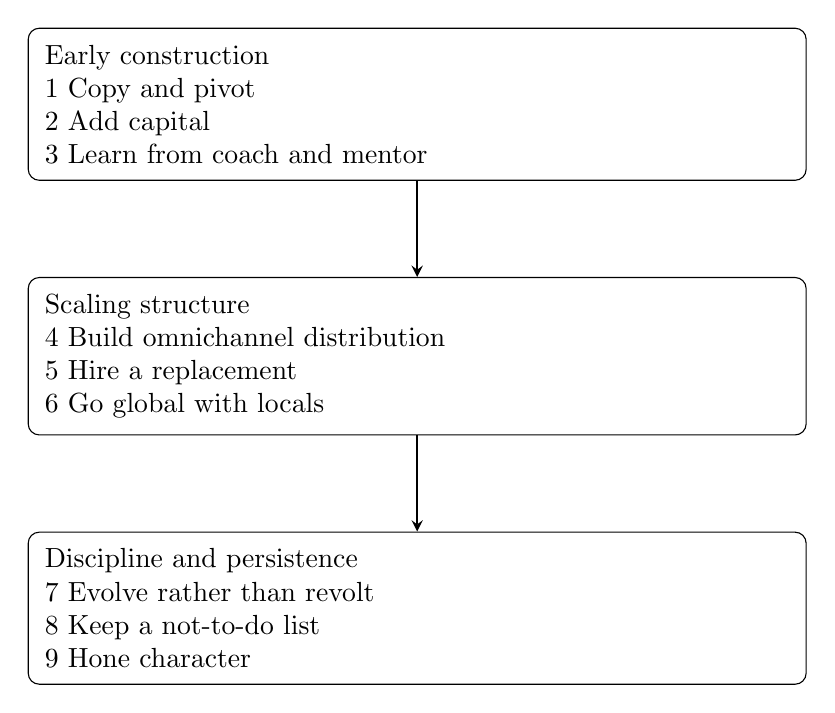
\begin{tikzpicture}[>=stealth]
\node[draw, rounded corners, align=left, text width=0.78\textwidth, inner sep=6pt] (a) at (0,0) {Early construction\\\(1\) Copy and pivot\\\(2\) Add capital\\\(3\) Learn from coach and mentor};
\node[draw, rounded corners, align=left, text width=0.78\textwidth, inner sep=6pt] (b) at (0,-3.2) {Scaling structure\\\(4\) Build omnichannel distribution\\\(5\) Hire a replacement\\\(6\) Go global with locals};
\node[draw, rounded corners, align=left, text width=0.78\textwidth, inner sep=6pt] (c) at (0,-6.4) {Discipline and persistence\\\(7\) Evolve rather than revolt\\\(8\) Keep a not-to-do list\\\(9\) Hone character};
\draw[->, thick] (a.south) -- (b.north);
\draw[->, thick] (b.south) -- (c.north);
\end{tikzpicture}
\caption{A transcript-based compression of the nine-step sequence.}
\end{figure}

The notes can also formalize one of Harpin's most concrete financing claims. Later, when he advises young entrepreneurs to buy a retiring owner's business and pay over three or four years from future profits, the compact mathematical summary is
\begin{equation}
P_{\mathrm{acq}} \approx \sum_{t=1}^{n}\pi_t,
\qquad
n\in\{3,4\},
\end{equation}
where \(P_{\mathrm{acq}}\) is the acquisition price and \(\pi_t\) is the profit available for payment in year \(t\). This is not a quoted formula from the lecture. It is a cautious compression of the spoken mechanism called vendor finance.

The algorithm is followed by the lecture's first clear moral answer to its title question. Harpin says that he did pay a large amount in tax and that, in his view, billionaires should pay their taxes, provided the regime remains relatively low and affordable. The lecture is careful here: the claim is neither anti-tax absolutism nor naive celebration of high rates. It is a compatibility claim between large-scale enterprise and ordinary civic obligation.

\section{Interlude, Waves, and the Geometry of Proximity}

After Harpin, the lecture briefly interrupts its main line with a promotional interlude. That interruption should not disappear from the notes, but it should be compressed. Even here the lecture keeps using numbers to dramatize access: a \(460\)-million-dollar sale, a company supposedly grown from zero to \(500\) million in less than five years and sold for \(2\) billion, and a private-equity billionaire who buys and scales companies. The interruption is part advertisement, part reinforcement of scale.

When the lecture returns to the street, it does not merely repeat Harpin's lesson. The Russian entrepreneur introduces a different mechanism. He traces his turning point to the collapse of the Soviet Union, the opening of trade, rising oil prices, and the sudden popularity of mobile phones. The phrase that matters is simple: we just catch the wave.

Here the central number is identified as revenue:
\begin{equation}
R_{2008} \approx 5\times 10^{9}\ \mathrm{USD}.
\end{equation}
The transcript is explicit on this point, and the notes should be equally explicit. Revenue is not profit, and it is not personal wealth. But the number still matters because it anchors the claim that historical timing and product popularity can generate scale very quickly.

The lecture also extracts a geometric principle. The host asks for a quick masterclass on how money works, and the answer begins with location. One should be in the right place; one should look around at the cars, the customers, the concentration of already-rich people. That logic is later restated by the host as ``proximity is power.'' It is not a full theory of wealth, but it is a recurring spatial motif in this lecture: when access, customers, or capital are unevenly distributed, location becomes part of the mechanism rather than mere scenery.

\section{Case Study IV: Cost, Family, and Tax Residence}

The final interview adds the chapter's cleanest piece of business arithmetic. The interviewee insists that cost management is more important than top-line boasting. The statement can be written in the simplest possible form:
\begin{equation}
m=p-c,
\end{equation}
where \(p\) is unit selling price, \(c\) is unit cost, and \(m\) is unit margin.

The lecture then supplies a worked example. If a product sells for \(10\) dollars and costs \(8\) dollars to obtain, then the margin is only \(2\):
\begin{equation}
m(10,8)=10-8=2.
\end{equation}
Now reduce the cost base while keeping pricing flexibility:
\begin{align}
m(5,2)&=5-2=3,\\
m(7,2)&=7-2=5,\\
m(10,2)&=10-2=8.
\end{align}
This is a small calculation, but it does real pedagogical work. The lecture's point is not merely that higher margins are better. It is that lower costs widen the set of market conditions under which one can survive and still sell.

\paragraph{Worked derivation.}
\begin{enumerate}
\item Start with the identity \(m=p-c\).
\item Hold the initial selling price at \(p=10\) and the initial cost at \(c=8\).
\item Compute the first margin: \(m=2\).
\item Lower the cost to \(c=2\).
\item Recompute margin at several possible selling prices \(p=5,7,10\).
\item Observe that cost control creates pricing freedom: one can accept a lower market price without collapsing margin altogether.
\end{enumerate}

But the final case does not stop at arithmetic. It moves through the difficulty of working with family, the need to distinguish father from partner, and the strain imposed by trials and setbacks. Then the lecture returns one last time to taxes. This time, however, the answer differs sharply from Harpin's. Residence in the UAE is presented as the decisive structural fact. The claim is that the family did not face the same exit-tax burden they would have faced in Britain.

\subsection{Question \& Answer}

\paragraph{Question.} Does the lecture end with a single answer to the question of whether billionaires pay taxes?

\paragraph{Answer.} No. It ends with a contrast. Harpin says that he paid nearly one hundred million pounds in tax and that paying tax is part of the social compact of wealth. The final interviewee treats tax exposure as something heavily shaped by jurisdiction and residence. The chapter should preserve that tension. The lecture does not offer a theorem of taxation. It offers reported entrepreneurial positions arranged so that the reader must keep both ethics and structure in view.

\section{Summary}

The lecture begins as a street spectacle and ends as a compact map of business mechanisms. First, London is framed as a high-tax environment, and taxation is introduced through a rough but forceful heuristic. Then access becomes a methodological problem, solved narratively by moving to a denser geography of wealth. The jeweler gives us a model of hustle, reputation, and cycle timing. Harpin supplies the lecture's most formal object, a nine-step business algorithm, and pairs it with a defense of paying taxes. The Russian entrepreneur adds timing, macro disruption, and proximity to the map. The final interview compresses the chapter into one clean margin equation and one unresolved tax contrast.

There is no blackboard here, but there is structure. Revenue is not earnings, earnings are not valuation, valuation is not tax paid, and tax paid is not a complete statement of civic virtue. Once we keep those distinctions alive, the lecture stops being a pile of luxury anecdotes and becomes a sequence of commercial models under pressure.